\documentclass[12pt,a4paper]{article}
\usepackage[utf8]{inputenc}
\usepackage[french]{babel}
\usepackage[T1]{fontenc}
\usepackage{graphicx}
\usepackage{listings}
\usepackage{float}
\usepackage{xcolor}
\usepackage{hyperref}
\usepackage{geometry}
\geometry{margin=2.5cm}

% --- Configuration du style pour les commandes Git ---
\lstset{
    language=bash,
    backgroundcolor=\color{gray!5},
    basicstyle=\footnotesize\ttfamily,
    keywordstyle=\color{blue},
    commentstyle=\color{green!60!black},
    frame=single,
    breaklines=true,
    captionpos=b
}

\title{Rapport de Mini-Projet : Gestion de Projet et Développement d'un Convertisseur Web Collaboratif}
\author{Licence Informatique 2A - Université Lyon 2 \\ Groupe de TD [X]}
\date{16 Mars 2026}

\begin{document}

\maketitle
\tableofcontents
\newpage

\section{Section 1 : Introduction / Contexte}

\subsection{Composition du groupe}
Le projet a été mené par une équipe de 4 étudiants, permettant une répartition des rôles proche d'un environnement professionnel :
\begin{itemize}
    \item \textbf{Ryan Bouteraa } - [5232973] 
    \item \textbf{Samy Adouda } - [N° Étudiant] 
    \item \textbf{Adam Rafa } - [N° Étudiant] 
    \item \textbf{Mohammed Geroli } - [N° Étudiant] 
\end{itemize}

\subsection{Sujet du projet}
Nous avons développé un \textbf{Convertisseur d'Unités Universel}. Ce projet de programmation utilise le trio HTML/CSS/JavaScript pour offrir une interface fluide capable de convertir des longueurs, des poids et des températures en temps réel. Ce support a été idéal pour expérimenter la gestion de version sur des fichiers interdépendants.

\subsection{Nom du dépôt en ligne :} 
\textbf{GitHub :} \url{https://github.com/zetsugax/Convertisseur} 



\section{Section 2 : Description des mises en situation}

\subsection{[A1] Constitution du groupe et [A2] Dépôt Git}
Nous avons instauré une communication via un canal dédié pour coordonner nos sessions de travail. Le dépôt a été initialisé sur Git Bash puis synchronisé avec GitHub.
\begin{figure}[H]
    \centering
    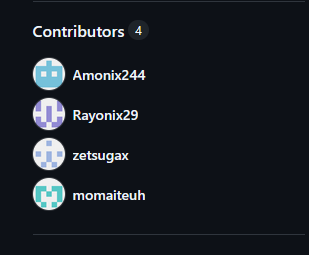
\includegraphics[width=0.8\textwidth]{image 1.png}
    \caption{Onglet Contributors GitHub}
    \label{fig:depot_git}
\end{figure}


\begin{figure}[H]
    \centering
    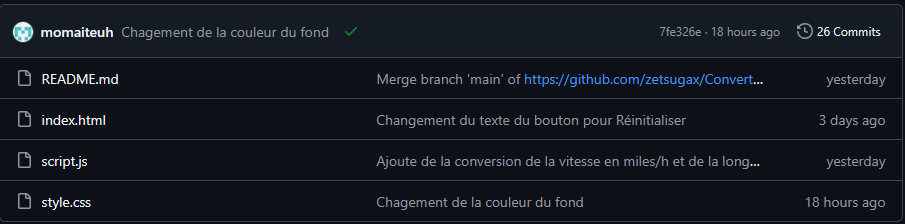
\includegraphics[width=0.8\textwidth]{image 2.png}
    \caption{Page d'accueil du dépôt avec les fichiers script.js, style.css}
    \label{fig:depot_git}
\end{figure}






\subsection{[A3] Intégration des contributions et Flux quotidien}
Le travail a été rythmé par des mises à jour quotidiennes. Chaque session de code suivait rigoureusement ce cycle de commandes pour éviter les désynchronisations :
\begin{lstlisting}[caption=Routine de sauvegarde quotidienne]
git status                # Verification des fichiers modifies
git add .                 # Indexation des changements
git commit -m "Message"   # Creation du point de sauvegarde
git pull                  # Recuperation du travail des autres
git push                  # Envoi sur le serveur
\end{lstlisting}
\textit{[Capture d'écran n°3 : Historique des commits montrant les différents auteurs]}

\subsection{[B1] Gestion par branches et Résolution de conflit}
Lors de la fusion de la branche JavaScript vers la branche principale, nous avons dû valider un commit de fusion (Merge Commit) via l'éditeur Vim, après avoir résolu un rejet de poussée (Push Rejected) \texttt .

\begin{figure}[H]
    \centering
    % Image 1 : 
    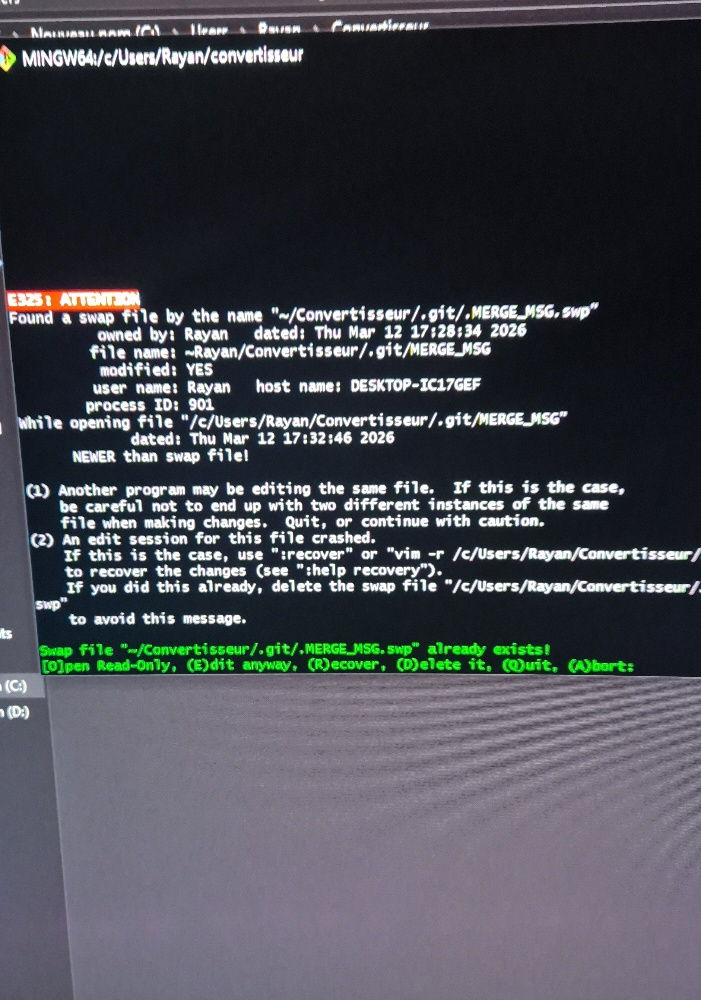
\includegraphics[width=0.3\textwidth]{image 3.jpg} \hfill
    % Image 2 : 
    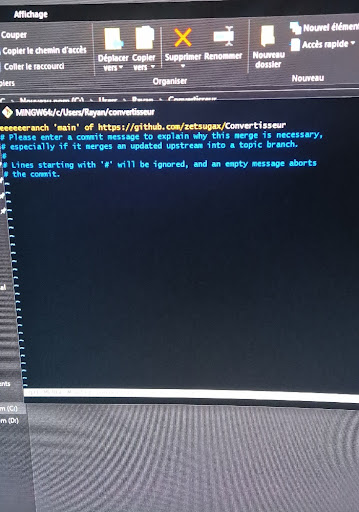
\includegraphics[width=0.3\textwidth]{image 4.jpg} \hfill
    % Image 3 : 
    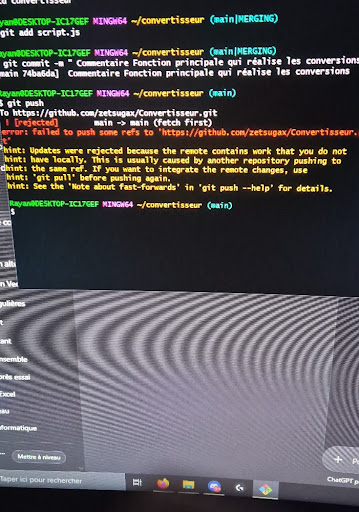
\includegraphics[width=0.3\textwidth]{image 5.jpg} 
    % Image 4 : 
    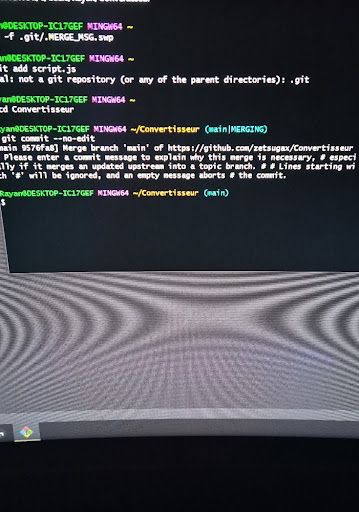
\includegraphics[width=0.3\textwidth]{image 6.jpg}
    
    \caption{Différents états d'erreurs et de blocages rencontrés sur Git (Vim et Push rejected).}
    \label{fig:erreurs_git}
\end{figure}

\textbf{Mise en situation :} Le terminal s'est retrouvé bloqué dans l'éditeur \textbf{Vim} suite à un conflit. Pour sortir de cet état, nous avons dû forcer la fermeture de l'éditeur , supprimer le fichier temporaire  (\texttt{.git/.MERGE\_MSG.swp}) et finaliser la fusion avec la commande :
\begin{lstlisting}
git commit --no-edit
\end{lstlisting}

\subsection{[B3] Pull Requests et [B4] Déploiement}
Chaque ajout majeur a fait l'objet d'une \textit{Pull Request}. Ce système nous a permis de relire le code (Code Review) avant l'intégration finale. Enfin, le site a été déployé via \textbf{GitHub Pages}.
\textbf{URL du site :} \url{https://zetsugax.github.io/Convertisseur/}
\textit{[Capture d'écran n°5 : Pull Request validee / Capture n°6 : Site en ligne]}

\subsection{[C1] Issues et [C4] GitHub Projects (Kanban)}
L'organisation des tâches a été gérée via l'onglet \textbf{Issues}, chaque ticket étant assigné à un membre. Ces tickets ont été pilotés graphiquement via un tableau \textbf{Kanban} dans GitHub Projects, permettant de suivre les colonnes \textit{Todo}, \textit{In Progress} et \textit{Done}.
\textit{[Capture d'écran n°7 : Liste des Issues / Capture n°8 : Tableau Kanban]}

\section{Section 3 : Conclusion}

\subsection{Bilan du projet}
Ce projet a été particulièrement formateur, non seulement pour la programmation JavaScript, mais surtout pour l'apprentissage du travail collaboratif. Nous avons appris qu'une gestion rigoureuse des branches et des messages de commit est indispensable pour éviter de perdre du temps sur des conflits de fichiers évitables.

\subsection{Difficultés et regrets}
La principale difficulté a été la gestion des outils en ligne de commande (Vim, Rebase). Nous avons notamment appris à utiliser \texttt{git pull --rebase} pour résoudre les rejets de \texttt{push} de manière propre. Notre seul regret est de ne pas avoir utilisé les \textit{Issues} dès le lancement du projet, ce qui aurait permis une planification encore plus fine dès la phase de conception.

\end{document}